\documentclass[12pt]{article}
\usepackage{amsmath}
\usepackage{graphicx}
\usepackage{hyperref}
\usepackage{listings}
\usepackage{color}
\usepackage{pythonhighlight}

\title{Operating System Course Report - First Half of the Semester}
\author{A class}
\date{\today}

\begin{document}

\maketitle
\newpage

\tableofcontents
\newpage

\section{Introduction}
This report summarizes the topics covered during the first half of the Operating System course. It includes theoretical concepts, practical implementations, and assignments. The course focuses on the fundamentals of operating systems, including system architecture, process management, CPU scheduling, and deadlock handling.

\section{Course Overview}
\subsection{Objectives}
The main objectives of this course are:
\begin{itemize}
    \item To understand the basic components and architecture of a computer system.
    \item To learn process management, scheduling, and inter-process communication.
    \item To explore file systems, input/output management, and virtualization.
    \item To study the prevention and handling of deadlocks in operating systems.
\end{itemize}

\subsection{Course Structure}
The course is divided into two halves. This report focuses on the first half, which covers:
\begin{itemize}
    \item Basic Concepts and Components of Computer Systems
    \item System Performance and Metrics
    \item System Architecture of Computer Systems
    \item Process Description and Control
    \item Scheduling Algorithms
    \item Process Creation and Termination
    \item Introduction to Threads
    \item File Systems
    \item Input and Output Management
    \item Deadlock Introduction and Prevention
    \item User Interface Management
    \item Virtualization in Operating Systems
\end{itemize}

\section{Topics Covered}

\subsection{Basic Concepts and Components of Computer Systems}
This section explains the fundamental components that make up a computer system, including the CPU, memory, storage, and input/output devices.

\subsection{System Performance and Metrics}
This section introduces various system performance metrics used to measure the efficiency of a computer system, including throughput, response time, and utilization.

\subsection{System Architecture of Computer Systems}
Describes the architecture of modern computer systems, focusing on the interaction between hardware and the operating system.

\subsection{Process Description and Control}
Processes are a central concept in operating systems. This section covers:
\begin{itemize}
    \item Process states and state transitions
    \item Process control block (PCB)
    \item Context switching
\end{itemize}

\subsection{Scheduling Algorithms}
This section covers:
\begin{itemize}
    \item First-Come, First-Served (FCFS)
    \item Shortest Job Next (SJN)
    \item Round Robin (RR)
\end{itemize}
It explains how these algorithms are used to allocate CPU time to processes.

\subsection{Process Creation and Termination}
Details how processes are created and terminated by the operating system, including:
\begin{itemize}
    \item Process spawning
    \item Process termination conditions
\end{itemize}

\subsection{Introduction to Threads}
This section introduces the concept of threads and their relation to processes, covering:
\begin{itemize}
    \item Konsep Threads
    \item Hubungan antara Threads dan Proses
    \item Manfaat Penggunaan Threads
    \item Multithreading
    \item Threads vs Process
    \item Model Multithreading
    \item Pengelolaan Threads
    \item Penerapan Threads pada Sistem Operasi
\end{itemize}
Penjelasannya dibawah ini:
\subsubsection{Konsep Threads}
\subsubsection{Hubungan antara Threads dan Proses}
\subsubsection{Manfaat Penggunaan Threads}
\subsubsection{\textit{Multithreading}}
Multithreading adalah teknik yang memungkinkan sebuah proses menjalankan beberapa tugas secara paralel dalam satu waktu. Setiap tugas ini disebut \textit{thread}, dan masing-masing \textit{thread} dapat berjalan secara independen, tetapi tetap berbagi sumber daya seperti memori dan file yang sama. Multithreading sangat berguna dalam meningkatkan efisiensi dan performa sebuah aplikasi, terutama untuk program yang perlu menangani banyak tugas bersamaan.

Dalam sistem operasi modern, multithreading digunakan untuk menjalankan proses-proses berat seperti pengolahan data atau menjalankan banyak aplikasi sekaligus, dengan memanfaatkan kemampuan prosesor untuk menangani beberapa pekerjaan secara simultan. Berikut beberapa konsep penting dalam multithreading:

\begin{itemize}
    \item \textbf{Keuntungan Multithreading}: Salah satu keuntungan utama dari multithreading adalah efisiensi. Dengan membagi tugas menjadi beberapa \textit{threads}, kita bisa memanfaatkan waktu tunggu saat satu \textit{thread} menunggu hasil dari operasi I/O (seperti membaca file) dengan menjalankan \textit{thread} lain. Hal ini membuat aplikasi lebih responsif dan cepat.

    \item \textbf{Konteks Berbagi Sumber Daya}: \textit{Threads} dalam satu proses berbagi memori yang sama, sehingga mereka dapat bekerja sama dengan lebih mudah dibandingkan proses-proses terpisah. Namun, karena berbagi sumber daya, kita juga harus memastikan tidak ada \textit{thread} yang saling mengganggu saat mengakses data yang sama. Ini bisa menyebabkan masalah seperti \textit{race conditions}, di mana hasil akhir dari suatu proses tergantung pada urutan eksekusi \textit{threads}.

    \item \textbf{Sinkronisasi \textit{Threads}}: Untuk mengatasi masalah dalam berbagi sumber daya, diperlukan mekanisme sinkronisasi. Contohnya, \textit{mutex} dan \textit{semaphore} digunakan untuk memastikan bahwa hanya satu \textit{thread} yang dapat mengakses bagian tertentu dari memori atau data pada satu waktu. Dengan cara ini, kita bisa mencegah konflik dan memastikan data tetap konsisten meskipun diakses oleh beberapa \textit{threads}.

    \item \textbf{Skalabilitas Multithreading}: Dalam sistem multithreaded, kita bisa memanfaatkan sepenuhnya kemampuan prosesor multi-core. Misalnya, jika sebuah program memiliki empat \textit{threads} dan dijalankan di komputer dengan prosesor empat inti, setiap \textit{thread} bisa berjalan di intinya masing-masing secara bersamaan, yang meningkatkan performa secara signifikan. Namun, manajemen \textit{threads} juga memerlukan pengelolaan yang baik untuk memastikan tidak terjadi \textit{overhead} yang malah memperlambat kinerja aplikasi.

    \item \textbf{Tantangan dalam Multithreading}: Meskipun multithreading dapat meningkatkan performa, teknik ini juga menimbulkan tantangan. Salah satunya adalah debugging, karena perilaku aplikasi multithreaded bisa menjadi sulit diprediksi. Kesalahan seperti \textit{deadlock} atau \textit{race conditions} sering kali sulit ditemukan, karena mereka mungkin tidak selalu muncul pada setiap eksekusi program. Oleh karena itu, pengembangan aplikasi multithreaded memerlukan perhatian khusus untuk memastikan bahwa semua \textit{threads} berjalan dengan aman dan efisien.
\end{itemize}

Dengan mengimplementasikan multithreading, kita bisa menciptakan aplikasi yang lebih efisien dan responsif, terutama ketika menangani tugas-tugas yang kompleks dan memerlukan pemrosesan paralel. Namun, seperti halnya teknologi lainnya, multithreading juga memerlukan perencanaan dan pengelolaan yang matang untuk memastikan hasil yang optimal.

\subsubsection{Threads vs Process}
\subsubsection{Model \textit{Multithreading}}
\textit{Multithreading} adalah fitur dari sistem operasi yang memungkinkan beberapa thread berjalan secara bersamaan dalam satu proses.
Ada beberapa model \textit{Multithreading} umumnya dibagi menjadi tiga, yaitu:
\begin{enumerate}
    \item Many-to-One Model (Banyak ke Satu)\\
    Pada model ini, banyak \textit{thread} yang dibuat oleh aplikasi \textit{(user-level)} dipetakan ke satu \textit{thread} di \textit{kernel}. Artinya, sistem operasi hanya melihat satu \textit{thread kernel} meskipun ada banyak \textit{thread} di tingkat aplikasi.
    Bayangkan kamu punya banyak tugas \textit{(thread user)} yang dikerjakan secara bergantian oleh satu orang \textit{(thread kernel)}. Orang tersebut harus menyelesaikan satu tugas sebelum beralih ke tugas lainnya, jadi jika satu tugas terhenti, semua tugas lain ikut tertunda.
    \begin{figure}[h]
        \centering
        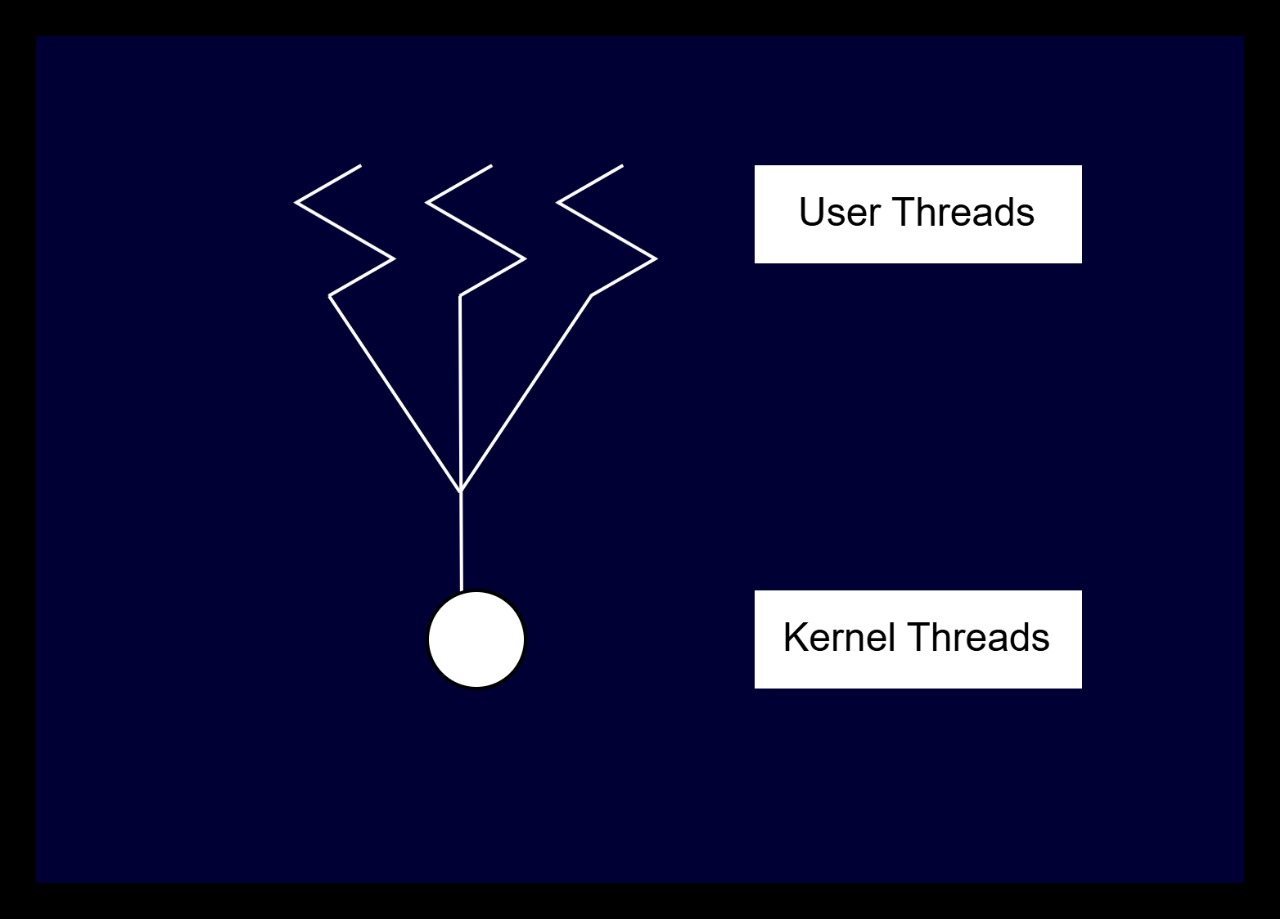
\includegraphics[width=0.5\textwidth]{asset/gambar-model-multithreading-many-to-one.jpg}
        \caption{Gambar Model \textit{Many-to-one}}
    \end{figure}
    \begin{itemize}
        \item Keuntungan \\
            \begin{enumerate}
                \item Lebih cepat dan efisien \\
                    Karena semua manajemen \textit{thread} terjadi di tingkat aplikasi, tidak perlu 
                    berkomunikasi dengan \textit{kernel}. Ini mengurangi waktu yang dibutuhkan untuk membuat, menghancurkan, atau mengubah \textit{thread}.
                \item Sederhana \\
                    Mudah diimplementasikan karena \textit{kernel} hanya perlu mengelola satu \textit{thread}, terlepas dari berapa banyak \textit{thread} yang 
                    dibuat oleh aplikasi.
            \end{enumerate}

        \item Kekurangan \\
            \begin{enumerate}
                \item Pemblokiran total \\
                Jika satu \textit{thread} terblokir (misalnya saat menunggu input), 
                seluruh proses akan berhenti, karena \textit{kernel} hanya bisa menangani satu \textit{thread}.
                \item Tidak cocok untuk multiprosesor \\
                Semua \textit{thread} dijalankan oleh satu \textit{thread kernel}, jadi meskipun ada banyak prosesor, hanya satu yang bisa 
                digunakan. Ini membuat model ini kurang efisien di sistem dengan banyak prosesor.
            \end{enumerate}
    \end{itemize}


    
    \item One-to-One Model (Satu ke Satu)\\
    Dalam model ini, setiap \textit{thread} yang dibuat di tingkat aplikasi dipetakan langsung ke satu \textit{thread kernel.}
    Jadi, untuk setiap \textit{thread user-level}, \textit{kernel} membuat satu \textit{thread} untuk mengelolanya.
    Bayangkan kamu punya banyak tugas \textit{(thread user)}, dan setiap tugas dikerjakan 
    oleh orang yang berbeda \textit{(thread kernel)}. Jika satu orang terhenti, yang lain tetap bisa bekerja, sehingga tugas-tugas lainnya tidak terganggu.
    \begin{figure}[h]
        \centering
        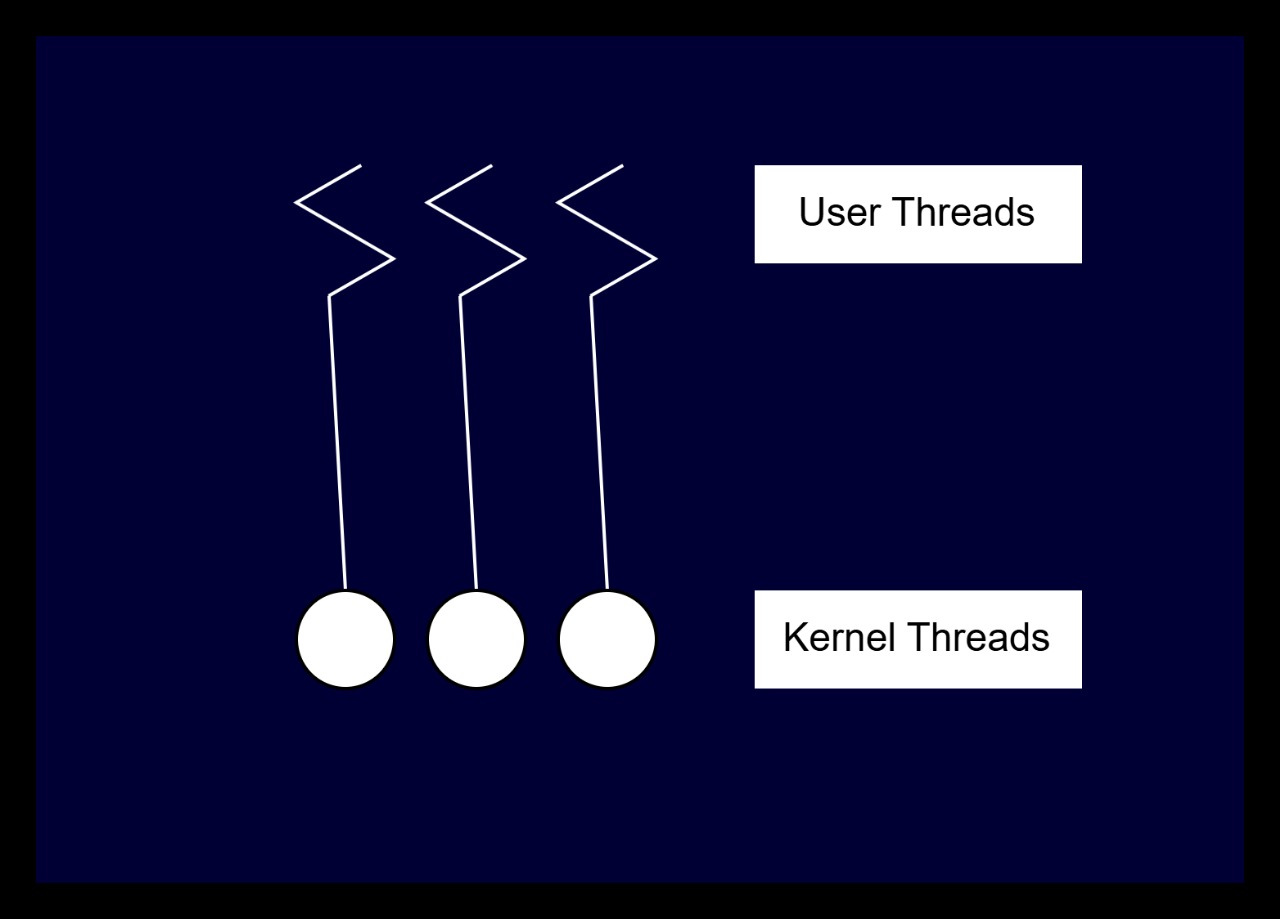
\includegraphics[width=0.5\textwidth]{asset/gambar-model-multithreading-one-to-one.jpg}
        \caption{Gambar Model \textit{One-to-one}}
    \end{figure}

    \begin{itemize}
        \item Keuntungan \\
        \begin{enumerate}
            \item Paralelisme lebih baik \\
                Setiap \textit{thread user-level} bisa berjalan secara paralel di prosesor yang berbeda, sehingga sistem multiprosesor bisa dimanfaatkan lebih baik.
            \item Tidak ada pemblokiran total \\
                Jika satu \textit{thread} terblokir, \textit{thread} lainnya masih bisa berjalan, karena masing-masing \textit{thread user-lever} dikelola oleh \textit{thread kernel} yang terpisah.
        \end{enumerate}
        \item Kekurangan \\
        \begin{enumerate}
            \item Overhead lebih besar \\
                Membuat \textit{thread kernel} untuk setiap \textit{thread user-level} membutuhkan lebih banyak memori dan sumber daya sistem. Jika ada banyak \textit{thread}, beban kerja untuk sistem operasi bisa 
                meningkat drastis.
            \item Switching antar \textit{thread} lebih lambat \\
                Karena setiap perpindahan \textit{(switching)} antar \textit{thread} harus melibatkan \textit{kernel}, ini membuat waktu \textit{switching} lebih lambat dibanding model \textit{many-to-one}.
        \end{enumerate}
    \end{itemize}

    \item Many-to-Many Model (Banyak ke Banyak)\\
    Model ini mengizinkan banyak \textit{thread user-level} 
    untuk dipetakan ke sejumlah \textit{thread kernel-level}. Dengan kata lain, 
    beberapa \textit{thread user-level} dapat dijalankan oleh beberapa 
    \textit{thread kernel-level}.
    \begin{figure}[h]
        \centering
        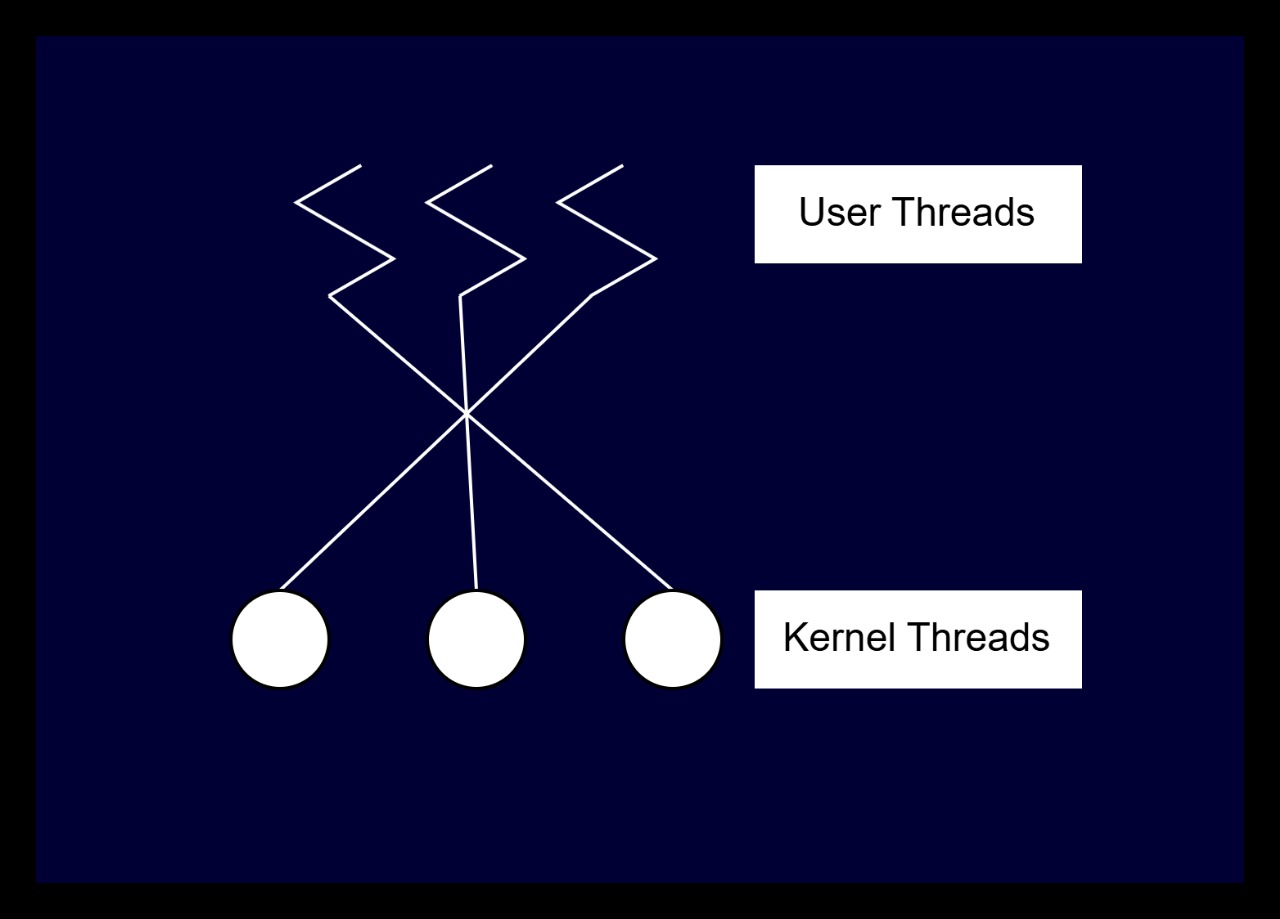
\includegraphics[width=0.5\textwidth]{asset/gambar-model-multithreading-many-to-many.jpg}
        \caption{Gambar Model \textit{Many-to-Many}}
    \end{figure}
    \begin{itemize}
        \item Keuntungan \\
            \begin{enumerate}
                \item Efisiensi dan fleksibilitas \\
                Kamu bisa memiliki lebih banyak \textit{thread user-level} daripada \textit{thread kernel-level}. Jadi, 
                \textit{thread-thread user-level} tidak harus selalu dihubungkan satu-satu ke \textit{thread kernel}, memungkinkan penggunaan sumber daya yang 
                lebih efisien
                \item Pemanfaatan multiprosesor \\
                Seperti model \textit{one-to-one, thread user-level} dapat berjalan secara paralel di banyak prosesor, 
                namun lebih hemat sumber daya karena tidak semua \textit{thread user} harus memiliki \textit{thread kernel} masing-masing.
            \end{enumerate}
        \item Kekurangan \\
            \begin{enumerate}
                \item Kompleksitas manajemen \\
                Model ini membutuhkan mekanisme yang lebih rumit untuk memetakan \textit{thread user-level} ke \textit{thread kernel-level}, dan bisa 
                jadi lebih sulit diimplementasikan.
                \item Potensi \textit{bottleneck} \\
                Jika terlalu banyak \textit{thread user} yang dipetakan ke \textit{thread kernel} yang sama, ini bisa menimbulkan kemacetan \textit{(bottleneck)} yang memperlambat performa.
            \end{enumerate}
    \end{itemize}

\end{enumerate}

\subsubsection{Pengelolaan \textit{Threads}}
Pengelolaan \textit{threads} merupakan salah satu aspek penting dalam sistem operasi untuk memastikan bahwa \textit{threads} dapat berjalan secara efisien dan tidak saling mengganggu. Sistem operasi bertanggung jawab untuk mengalokasikan waktu CPU, memori, serta sumber daya lain bagi setiap \textit{thread}. Berikut adalah beberapa elemen utama dalam pengelolaan \textit{threads}:

\begin{itemize}
    \item \textbf{Pembuatan \textit{Threads}}: Sistem operasi memungkinkan aplikasi untuk membuat \textit{threads} baru saat dibutuhkan. Misalnya, saat sebuah aplikasi memulai tugas paralel, sistem operasi akan membuat satu atau lebih \textit{threads} untuk menangani tugas-tugas tersebut. Setiap \textit{thread} memiliki identitas unik dan dikaitkan dengan proses induknya. Pembuatan \textit{threads} biasanya dilakukan melalui API atau fungsi-fungsi khusus yang disediakan oleh sistem operasi, seperti \texttt{pthread\_create()} pada \textit{Linux} atau \texttt{CreateThread()} pada \textit{Windows}.

    \item \textbf{Penjadwalan \textit{Threads}}: Sistem operasi menggunakan algoritma penjadwalan untuk menentukan urutan eksekusi \textit{threads}. Ini memastikan bahwa \textit{threads} dari berbagai proses mendapatkan waktu CPU secara adil dan efisien. Beberapa algoritma penjadwalan yang digunakan dalam pengelolaan \textit{threads} antara lain \textit{Round Robin} dan \textit{Priority Scheduling}. Penjadwalan yang baik sangat penting untuk menjaga kinerja sistem secara keseluruhan, terutama dalam lingkungan dengan banyak \textit{threads} yang berjalan bersamaan.

    \item \textbf{Sinkronisasi \textit{Threads}}: Ketika beberapa \textit{threads} berbagi sumber daya yang sama, sistem operasi harus memastikan bahwa tidak terjadi konflik saat \textit{threads} mengakses sumber daya tersebut. Mekanisme sinkronisasi seperti \textit{mutexes}, \textit{semaphores}, dan \textit{condition variables} digunakan untuk mengelola akses bersamaan dan mencegah kondisi balapan (\textit{race conditions}). Sinkronisasi memastikan bahwa \textit{threads} tidak saling mengganggu dan data yang digunakan tetap konsisten.

    \item \textbf{Penghentian \textit{Threads}}: Setelah \textit{threads} selesai menjalankan tugasnya, sistem operasi harus menghentikan \textit{threads} tersebut dan membersihkan sumber daya yang digunakan. Penghentian \textit{threads} dapat dilakukan secara manual oleh aplikasi, atau secara otomatis ketika tugas telah selesai. Fungsi-fungsi seperti \texttt{pthread\_exit()} pada \textit{Linux} atau \texttt{ExitThread()} pada \textit{Windows} digunakan untuk mengakhiri \textit{threads}.

    \item \textbf{Manajemen Konteks \textit{Threads}}: Ketika sistem operasi berpindah dari satu \textit{thread} ke \textit{thread} lainnya, perlu dilakukan penyimpanan dan pemulihan konteks eksekusi (\textit{context switching}). Konteks ini mencakup informasi tentang status CPU, register, dan memori yang sedang digunakan oleh \textit{thread}. Sistem operasi harus memastikan bahwa ketika sebuah \textit{thread} dilanjutkan, ia bisa melanjutkan eksekusinya tanpa kehilangan data atau instruksi penting.
\end{itemize}

Pengelolaan \textit{threads} yang efektif sangat penting untuk meningkatkan kinerja sistem operasi, terutama pada sistem dengan banyak tugas yang berjalan secara bersamaan. Dengan teknik yang tepat, \textit{threads} dapat membantu mempercepat penyelesaian tugas dan memastikan pemanfaatan sumber daya secara optimal.

\subsubsection{Penerapan \textit{Threads} pada Sistem Operasi}
Sistem operasi modern seperti \textit{Windows}, \textit{Linux}, dan \textit{macOS} menerapkan konsep \textit{threads} untuk meningkatkan efisiensi dan performa ketika menjalankan berbagai tugas secara bersamaan. Berikut adalah beberapa contoh penerapan \textit{threads} pada sistem operasi:

\begin{itemize}
    \item \textbf{\textit{Multitasking}}: Dalam sistem operasi, setiap proses atau aplikasi dapat terdiri dari beberapa \textit{threads} yang bekerja bersamaan. Misalnya, ketika kamu menjalankan \textit{browser}, mengetik dokumen, dan mendengarkan musik, sistem operasi menggunakan \textit{threads} untuk mengatur agar semua aplikasi tersebut bisa berjalan tanpa saling mengganggu. Setiap \textit{thread} diatur secara independen sehingga \textit{multitasking} dapat tercapai dengan lancar.
    
    \item \textbf{Pembagian Tugas dalam Aplikasi}: Banyak aplikasi modern menggunakan \textit{threads} untuk membagi tugas-tugas yang lebih kecil. Misalnya, dalam aplikasi peramban (\textit{browser}), satu \textit{thread} bisa bertanggung jawab untuk menampilkan halaman web, sementara \textit{thread} lain mengunduh gambar, dan \textit{thread} lainnya lagi mengelola animasi. Penggunaan \textit{threads} ini membuat aplikasi lebih responsif dan tidak bergantung pada satu proses untuk menyelesaikan semua tugas.
    
    \item \textbf{Penggunaan Sumber Daya yang Efisien}: Pada sistem dengan prosesor multi-core, sistem operasi dapat mendistribusikan \textit{threads} ke berbagai inti (\textit{core}). Ini memungkinkan proses berjalan secara paralel dan mempercepat kinerja sistem. Bayangkan sebuah tugas besar yang dibagi ke beberapa pekerja (\textit{thread}), masing-masing menyelesaikan bagian mereka secara bersamaan, sehingga tugas selesai lebih cepat.
    
    \item \textbf{\textit{Input/Output} (\textit{I/O} Operations)}: Ketika aplikasi menunggu input dari pengguna atau operasi \textit{I/O} seperti pembacaan file dari disk atau pengunduhan data dari internet, \textit{threads} lain masih bisa berjalan. Misalnya, saat menunggu halaman web dimuat, kamu tetap bisa menggulir halaman atau mengetik alamat baru karena ada \textit{thread} yang khusus menangani \textit{I/O} dan \textit{thread} lainnya yang tetap aktif untuk menerima interaksi pengguna.
\end{itemize}




\subsection{File Systems}
File systems provide a way for the operating system to store, retrieve, and manage data. This section explains:
\begin{itemize}
    \item File system structure
    \item File access methods
    \item Directory management
\end{itemize}

\subsection{Input and Output Management}
Input and output management is key for handling the interaction between the system and external devices. This section includes:
\begin{itemize}
    \item Device drivers
    \item I/O scheduling
\end{itemize}

\subsection{Deadlock Introduction and Prevention}
Explores the concept of deadlocks and methods for preventing them:
\begin{itemize}
    \item Deadlock conditions
    \item Deadlock prevention techniques
\end{itemize}

\subsection{User Interface Management}
This section discusses the role of the operating system in managing the user interface. Topics covered include:
\begin{itemize}
    \item Graphical User Interface (GUI)
    \item Command-Line Interface (CLI)
    \item Interaction between the user and the operating system
\end{itemize}

\subsection{Virtualization in Operating Systems}
Virtualization allows multiple operating systems to run concurrently on a single physical machine. This section explores:
\begin{itemize}
    \item Concept of virtualization
    \item Hypervisors and their types
    \item Benefits of virtualization in modern computing
\end{itemize}

\begin{figure}[h]
    \centering
    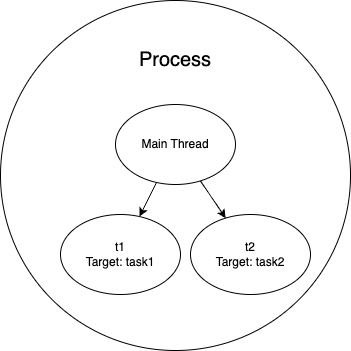
\includegraphics[width=0.5\textwidth]{/Users/khawaritzmi/Unhas/os_report_mid2024/a_class/asset/example.png}  % Sesuaikan nama file dan ukurannya
    \caption{Ini adalah gambar contoh dari multithreading.}
    \label{fig:contoh_gambar}
\end{figure}

Seperti yang terlihat pada Gambar \ref{fig:contoh_gambar}, inilah cara menambahkan gambar dengan keterangan.

\section{Assignments and Practical Work}
\subsection{Assignment 1: Process Scheduling}
Students were tasked with implementing various process scheduling algorithms (e.g., FCFS, SJN, and RR) and comparing their performance under different conditions.


\subsection{Assignment 2: Deadlock Handling}
In this assignment, students were asked to simulate different deadlock scenarios and explore various prevention methods.

\subsection{Assignment 3: Multithreading and Amdahl's Law}
This assignment involved designing a multithreading scenario to solve a computationally intensive problem. Students then applied **Amdahl's Law** to calculate the theoretical speedup of the program as the number of threads increased.

\subsection{Assignment 4: Simple Command-Line Interface (CLI) for User Interface Management}
Students were tasked with creating a simple **CLI** for user interface management. The CLI should support basic commands such as file manipulation (creating, listing, and deleting files), process management, and system status reporting.

\subsection{Assignment 5: File System Access}
In this assignment, students implemented file system access routines, including:
\begin{itemize}
    \item File creation and deletion
    \item Reading from and writing to files
    \item Navigating directories and managing file permissions
\end{itemize}

\section{Conclusion}
The first half of the course introduced core operating system concepts, including process management, scheduling, multithreading, and file system access. These topics provided a foundation for more advanced topics to be covered in the second half of the course.

\end{document}